\documentclass{standalone}
\usepackage{tikz}
\usetikzlibrary{patterns, positioning}


\begin{document}
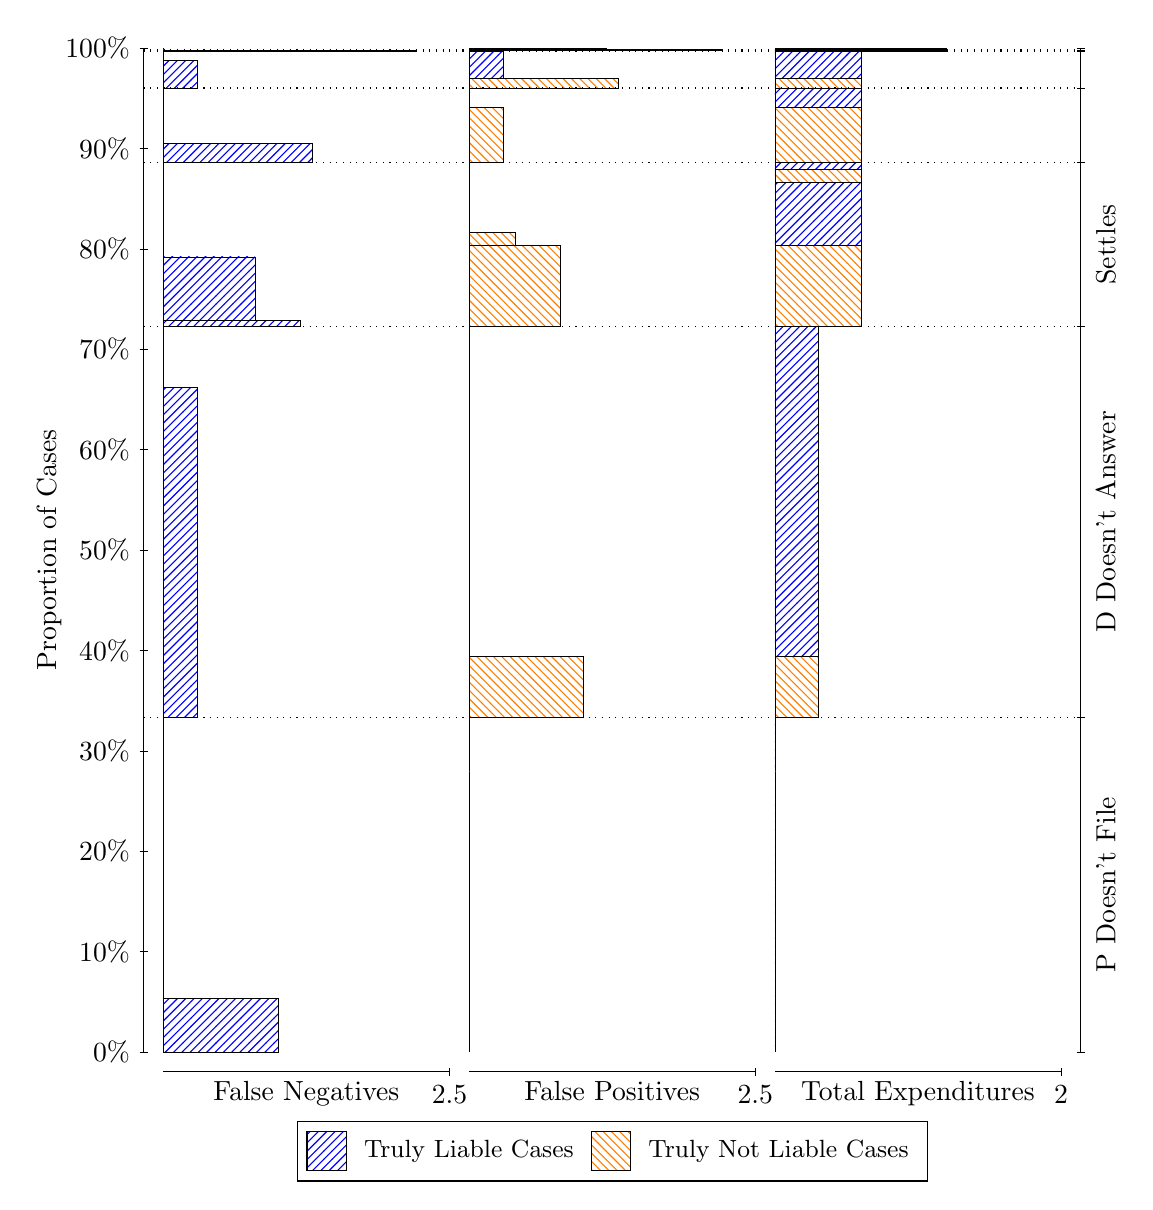
\begin{tikzpicture}
\draw[black, very thin] (1.5,1.75) -- (1.5,14.5);
\node[rotate=90, text=black, anchor=center] at (0.3, 8.125) {Proportion of Cases};
\draw[black, very thin] (1.45,1.75) -- (1.55,1.75);
\node[text=black, anchor=east] at (1.45, 1.75) {0\%};
\draw[black, very thin] (1.45,3.025) -- (1.55,3.025);
\node[text=black, anchor=east] at (1.45, 3.025) {10\%};
\draw[black, very thin] (1.45,4.3) -- (1.55,4.3);
\node[text=black, anchor=east] at (1.45, 4.3) {20\%};
\draw[black, very thin] (1.45,5.575) -- (1.55,5.575);
\node[text=black, anchor=east] at (1.45, 5.575) {30\%};
\draw[black, very thin] (1.45,6.85) -- (1.55,6.85);
\node[text=black, anchor=east] at (1.45, 6.85) {40\%};
\draw[black, very thin] (1.45,8.125) -- (1.55,8.125);
\node[text=black, anchor=east] at (1.45, 8.125) {50\%};
\draw[black, very thin] (1.45,9.4) -- (1.55,9.4);
\node[text=black, anchor=east] at (1.45, 9.4) {60\%};
\draw[black, very thin] (1.45,10.675) -- (1.55,10.675);
\node[text=black, anchor=east] at (1.45, 10.675) {70\%};
\draw[black, very thin] (1.45,11.95) -- (1.55,11.95);
\node[text=black, anchor=east] at (1.45, 11.95) {80\%};
\draw[black, very thin] (1.45,13.225) -- (1.55,13.225);
\node[text=black, anchor=east] at (1.45, 13.225) {90\%};
\draw[black, very thin] (1.45,14.5) -- (1.55,14.5);
\node[text=black, anchor=east] at (1.45, 14.5) {100\%};

\draw[black, very thin] (13.4,1.75) -- (13.4,14.5);
\draw[black, very thin] (13.35,1.75) -- (13.45,1.75);
\node[anchor=west] at (13.35, 1.75) {};
\draw[black, very thin] (13.35,5.9964) -- (13.45,5.9964);
\node[anchor=west] at (13.35, 5.9964) {};
\draw[black, very thin] (13.35,10.964) -- (13.45,10.964);
\node[anchor=west] at (13.35, 10.964) {};
\draw[black, very thin] (13.35,13.043) -- (13.45,13.043);
\node[anchor=west] at (13.35, 13.043) {};
\draw[black, very thin] (13.35,13.992) -- (13.45,13.992);
\node[anchor=west] at (13.35, 13.992) {};
\draw[black, very thin] (13.35,14.462) -- (13.45,14.462);
\node[anchor=west] at (13.35, 14.462) {};
\draw[black, very thin] (13.35,14.477) -- (13.45,14.477);
\node[anchor=west] at (13.35, 14.477) {};
\draw[black, very thin] (13.35,14.5) -- (13.45,14.5);
\node[anchor=west] at (13.35, 14.5) {};

\draw[black, very thin, pattern color=blue, pattern=north east lines] (1.75,1.75) rectangle (3.2033,2.432);
\draw[black, very thin, pattern color=orange, pattern=north west lines] (1.75,2.432) rectangle (1.75,5.9964);
\draw[black, very thin, pattern color=blue, pattern=north east lines] (1.75,5.9964) rectangle (2.186,10.187);
\draw[black, very thin, pattern color=orange, pattern=north west lines] (1.75,10.187) rectangle (1.75,10.964);
\draw[black, very thin, pattern color=blue, pattern=north east lines] (1.75,10.964) rectangle (3.494,11.045);
\draw[black, very thin, pattern color=blue, pattern=north east lines] (1.75,11.045) rectangle (2.9127,11.848);
\draw[black, very thin, pattern color=orange, pattern=north west lines] (1.75,11.848) rectangle (1.75,13.043);
\draw[black, very thin, pattern color=blue, pattern=north east lines] (1.75,13.043) rectangle (3.6393,13.288);
\draw[black, very thin, pattern color=orange, pattern=north west lines] (1.75,13.288) rectangle (1.75,13.992);
\draw[black, very thin, pattern color=blue, pattern=north east lines] (1.75,13.992) rectangle (2.186,14.344);
\draw[black, very thin, pattern color=orange, pattern=north west lines] (1.75,14.344) rectangle (1.75,14.462);
\draw[black, very thin, pattern color=blue, pattern=north east lines] (1.75,14.462) rectangle (4.9473,14.469);
\draw[black, very thin, pattern color=orange, pattern=north west lines] (1.75,14.469) rectangle (1.75,14.477);
\draw[black, very thin, pattern color=orange, pattern=north west lines] (1.75,14.477) rectangle (1.75,14.484);
\draw[black, very thin, pattern color=blue, pattern=north east lines] (1.75,14.484) rectangle (1.75,14.5);
\draw[black, very thin, pattern color=orange, pattern=north west lines] (5.6333,1.75) rectangle (5.6333,5.3144);
\draw[black, very thin, pattern color=blue, pattern=north east lines] (5.6333,5.3144) rectangle (5.6333,5.9964);
\draw[black, very thin, pattern color=orange, pattern=north west lines] (5.6333,5.9964) rectangle (7.0867,6.774);
\draw[black, very thin, pattern color=blue, pattern=north east lines] (5.6333,6.774) rectangle (5.6333,10.964);
\draw[black, very thin, pattern color=orange, pattern=north west lines] (5.6333,10.964) rectangle (6.796,11.994);
\draw[black, very thin, pattern color=orange, pattern=north west lines] (5.6333,11.994) rectangle (6.2147,12.16);
\draw[black, very thin, pattern color=blue, pattern=north east lines] (5.6333,12.16) rectangle (5.6333,13.043);
\draw[black, very thin, pattern color=orange, pattern=north west lines] (5.6333,13.043) rectangle (6.0693,13.748);
\draw[black, very thin, pattern color=blue, pattern=north east lines] (5.6333,13.748) rectangle (5.6333,13.992);
\draw[black, very thin, pattern color=orange, pattern=north west lines] (5.6333,13.992) rectangle (7.5227,14.11);
\draw[black, very thin, pattern color=blue, pattern=north east lines] (5.6333,14.11) rectangle (6.0693,14.462);
\draw[black, very thin, pattern color=orange, pattern=north west lines] (5.6333,14.462) rectangle (5.6333,14.471);
\draw[black, very thin, pattern color=blue, pattern=north east lines] (5.6333,14.471) rectangle (5.6333,14.477);
\draw[black, very thin, pattern color=orange, pattern=north west lines] (5.6333,14.477) rectangle (8.8307,14.484);
\draw[black, very thin, pattern color=blue, pattern=north east lines] (5.6333,14.484) rectangle (7.3773,14.5);
\draw[black, very thin, pattern color=orange, pattern=north west lines] (9.5167,1.75) rectangle (9.5167,5.3144);
\draw[black, very thin, pattern color=blue, pattern=north east lines] (9.5167,5.3144) rectangle (9.5167,5.9964);
\draw[black, very thin, pattern color=orange, pattern=north west lines] (9.5167,5.9964) rectangle (10.062,6.774);
\draw[black, very thin, pattern color=blue, pattern=north east lines] (9.5167,6.774) rectangle (10.062,10.964);
\draw[black, very thin, pattern color=orange, pattern=north west lines] (9.5167,10.964) rectangle (10.607,11.994);
\draw[black, very thin, pattern color=blue, pattern=north east lines] (9.5167,11.994) rectangle (10.607,12.797);
\draw[black, very thin, pattern color=orange, pattern=north west lines] (9.5167,12.797) rectangle (10.607,12.963);
\draw[black, very thin, pattern color=blue, pattern=north east lines] (9.5167,12.963) rectangle (10.607,13.043);
\draw[black, very thin, pattern color=orange, pattern=north west lines] (9.5167,13.043) rectangle (10.607,13.748);
\draw[black, very thin, pattern color=blue, pattern=north east lines] (9.5167,13.748) rectangle (10.607,13.992);
\draw[black, very thin, pattern color=orange, pattern=north west lines] (9.5167,13.992) rectangle (10.607,14.11);
\draw[black, very thin, pattern color=blue, pattern=north east lines] (9.5167,14.11) rectangle (10.607,14.462);
\draw[black, very thin, pattern color=orange, pattern=north west lines] (9.5167,14.462) rectangle (11.697,14.471);
\draw[black, very thin, pattern color=blue, pattern=north east lines] (9.5167,14.471) rectangle (11.697,14.477);
\draw[black, very thin, pattern color=orange, pattern=north west lines] (9.5167,14.477) rectangle (11.697,14.484);
\draw[black, very thin, pattern color=blue, pattern=north east lines] (9.5167,14.484) rectangle (11.697,14.5);
\draw[black, dotted] (1.5,5.9964) -- (13.4,5.9964);
\draw[black, dotted] (1.5,10.964) -- (13.4,10.964);
\draw[black, dotted] (1.5,13.043) -- (13.4,13.043);
\draw[black, dotted] (1.5,13.992) -- (13.4,13.992);
\draw[black, dotted] (1.5,14.462) -- (13.4,14.462);
\draw[black, dotted] (1.5,14.477) -- (13.4,14.477);
\draw[black, very thin] (1.75,1.5) -- (5.3833,1.5);
\node[text=black, anchor=north] at (3.5667, 1.5) {False Negatives};
\draw[black, very thin] (5.3833,1.45) -- (5.3833,1.55);
\node[text=black, anchor=north] at (5.3833, 1.45) {2.5};

\draw[black, very thin] (5.6333,1.5) -- (9.2667,1.5);
\node[text=black, anchor=north] at (7.45, 1.5) {False Positives};
\draw[black, very thin] (9.2667,1.45) -- (9.2667,1.55);
\node[text=black, anchor=north] at (9.2667, 1.45) {2.5};

\draw[black, very thin] (9.5167,1.5) -- (13.15,1.5);
\node[text=black, anchor=north] at (11.333, 1.5) {Total Expenditures};
\draw[black, very thin] (13.15,1.45) -- (13.15,1.55);
\node[text=black, anchor=north] at (13.15, 1.45) {2};

\node[text=black, centered, rotate=90] at (13.72, 3.8732) {P Doesn't File};
\node[text=black, centered, rotate=90] at (13.72, 8.4803) {D Doesn't Answer};
\node[text=black, centered, rotate=90] at (13.72, 12.004) {Settles};





\draw (7.449999999999999,1.5) node[draw=none] (baseCoordinate) {};
\begin{scope}[align=center]
        \matrix[scale=0.5, draw=black, below=0.5cm of baseCoordinate, nodes={draw}, column sep=0.1cm]{
            \node[rectangle, draw, minimum width=0.5cm, minimum height=0.5cm, pattern color=blue, pattern=north east lines] {}; &
            \node[draw=none, font=\small, text=black] (B) {Truly Liable Cases}; &
            \node[rectangle, draw, minimum width=0.5cm, minimum height=0.5cm, pattern color=orange, pattern=north west lines] {}; &
            \node[draw=none, font=\small, text=black] (B) {Truly Not Liable Cases}; \\
            };
\end{scope}

\end{tikzpicture}
\end{document}